% Whole-tumour population-graph manuscript. Every number in the text comes from tables/numbers.tex
% and every table and figure from scripts/make_assets.py, so a re-run updates the manuscript.

\documentclass[11pt,a4paper]{article}

\usepackage[a4paper,top=1.8cm,bottom=2cm,left=1.5cm,right=1.5cm]{geometry}
\usepackage[T1]{fontenc}
\usepackage[utf8]{inputenc}
\usepackage{lmodern}
\usepackage{microtype}
\usepackage{graphicx}
\usepackage{amsmath,amssymb}
\usepackage{booktabs}
\usepackage{xcolor}
\usepackage[font=small,labelfont=bf,skip=4pt]{caption}
\usepackage[compact,small]{titlesec}
\usepackage[numbers,sort&compress]{natbib}
\usepackage[hidelinks]{hyperref}

\graphicspath{{figures/}}
\newcommand{\ablPrimBurDMMax}{0.84}
\newcommand{\ablPrimBurDMMin}{0.65}
\newcommand{\ablPrimBurLRMax}{0.63}
\newcommand{\ablPrimBurLRMin}{0.58}
\newcommand{\ablPrimBurOSMax}{0.69}
\newcommand{\ablPrimBurOSMin}{0.65}
\newcommand{\ablPrimVolDMMax}{0.78}
\newcommand{\ablPrimVolDMMin}{0.65}
\newcommand{\ablPrimVolLRMax}{0.63}
\newcommand{\ablPrimVolLRMin}{0.58}
\newcommand{\ablPrimVolOSMax}{0.70}
\newcommand{\ablPrimVolOSMin}{0.65}
\newcommand{\ablTotBurDMMax}{0.87}
\newcommand{\ablTotBurDMMin}{0.85}
\newcommand{\ablTotBurLRMax}{0.63}
\newcommand{\ablTotBurLRMin}{0.59}
\newcommand{\ablTotBurOSMax}{0.73}
\newcommand{\ablTotBurOSMin}{0.70}
\newcommand{\ablTotVolDMMax}{0.88}
\newcommand{\ablTotVolDMMin}{0.85}
\newcommand{\ablTotVolLRMax}{0.63}
\newcommand{\ablTotVolLRMin}{0.58}
\newcommand{\ablTotVolOSMax}{0.73}
\newcommand{\ablTotVolOSMin}{0.72}
\newcommand{\clinOnlyDMMax}{0.81}
\newcommand{\clinOnlyDMMin}{0.79}
\newcommand{\clinOnlyLRMax}{0.57}
\newcommand{\clinOnlyLRMin}{0.51}
\newcommand{\clinOnlyOSMax}{0.70}
\newcommand{\clinOnlyOSMin}{0.69}
\newcommand{\clsAvail}{0}
\newcommand{\cnnDMCVClin}{0.88}
\newcommand{\cnnDMCVImg}{0.83}
\newcommand{\cnnDMCohClin}{0.93}
\newcommand{\cnnDMCohImg}{0.89}
\newcommand{\cnnLRCVClin}{0.57}
\newcommand{\cnnLRCVImg}{0.53}
\newcommand{\cnnLRCohClin}{0.59}
\newcommand{\cnnLRCohImg}{0.45}
\newcommand{\cnnOSCVClin}{0.68}
\newcommand{\cnnOSCVImg}{0.63}
\newcommand{\cnnOSCohClin}{0.69}
\newcommand{\cnnOSCohImg}{0.67}
\newcommand{\eTestDM}{7}
\newcommand{\eTestLR}{30}
\newcommand{\eTestOS}{45}
\newcommand{\figGraphK}{20}
\newcommand{\mainCIDMCohClin}{0.68--0.98}
\newcommand{\mainCIDMCohImg}{0.71--0.99}
\newcommand{\mainCILRCohClin}{0.46--0.72}
\newcommand{\mainCILRCohImg}{0.51--0.74}
\newcommand{\mainCIOSCohClin}{0.58--0.80}
\newcommand{\mainCIOSCohImg}{0.61--0.82}
\newcommand{\mainDMCVClin}{0.87}
\newcommand{\mainDMCVImg}{0.85}
\newcommand{\mainDMCohClin}{0.85}
\newcommand{\mainDMCohImg}{0.87}
\newcommand{\mainDMMax}{0.87}
\newcommand{\mainDMMin}{0.85}
\newcommand{\mainLRCVClin}{0.59}
\newcommand{\mainLRCVImg}{0.62}
\newcommand{\mainLRCohClin}{0.60}
\newcommand{\mainLRCohImg}{0.63}
\newcommand{\mainLRMax}{0.63}
\newcommand{\mainLRMin}{0.59}
\newcommand{\mainOSCVClin}{0.72}
\newcommand{\mainOSCVImg}{0.73}
\newcommand{\mainOSCohClin}{0.70}
\newcommand{\mainOSCohImg}{0.72}
\newcommand{\mainOSMax}{0.73}
\newcommand{\mainOSMin}{0.70}
\newcommand{\matchedN}{1944}
\newcommand{\matchedTestDeltaDM}{-0.006}
\newcommand{\matchedTestDeltaLR}{-0.002}
\newcommand{\matchedTestDeltaOS}{-0.010}
\newcommand{\matchedTestFracAll}{29}
\newcommand{\matchedTestFracDM}{26}
\newcommand{\matchedTestFracLR}{44}
\newcommand{\matchedTestFracOS}{14}
\newcommand{\matchedTestMedAll}{-0.006}
\newcommand{\matchedValFracAll}{34}
\newcommand{\matchedValFracDM}{22}
\newcommand{\matchedValFracLR}{55}
\newcommand{\matchedValFracOS}{34}
\newcommand{\mlpDMCVClin}{0.86}
\newcommand{\mlpDMCVImg}{0.85}
\newcommand{\mlpDMCohClin}{0.86}
\newcommand{\mlpDMCohImg}{0.86}
\newcommand{\mlpLRCVClin}{0.59}
\newcommand{\mlpLRCVImg}{0.59}
\newcommand{\mlpLRCohClin}{0.58}
\newcommand{\mlpLRCohImg}{0.64}
\newcommand{\mlpOSCVClin}{0.72}
\newcommand{\mlpOSCVImg}{0.74}
\newcommand{\mlpOSCohClin}{0.72}
\newcommand{\mlpOSCohImg}{0.73}
\newcommand{\nPatCan}{294}
\newcommand{\nPatMAA}{137}
\newcommand{\nTestDM}{109}
\newcommand{\nTestLR}{121}
\newcommand{\nTestOS}{135}
\newcommand{\nodalFracMedCan}{44}
\newcommand{\nodalFracMedMAA}{30}
\newcommand{\nodalPctCan}{37}
\newcommand{\nodalPctMAA}{59}
\newcommand{\pairedDeltaMax}{+0.050}
\newcommand{\pairedDeltaMin}{-0.023}
\newcommand{\pairedMinP}{0.03}
\newcommand{\pairedN}{18}
\newcommand{\pairedNsig}{1}
\newcommand{\seedRepeats}{1}
\newcommand{\seedSDmax}{nan}
\newcommand{\seedSDmed}{nan}
\newcommand{\seedStableLoss}{3}
\newcommand{\seedStableWins}{9}
\newcommand{\winsCls}{0}
\newcommand{\winsGraph}{9}
\newcommand{\winsMLP}{8}
\newcommand{\winsPrimBur}{7}
\newcommand{\winsPrimVol}{6}
\newcommand{\winsTotBur}{9}
\newcommand{\winsTotVol}{9}


\setlength{\parskip}{0pt}
\setlength{\textfloatsep}{10pt plus 2pt minus 3pt}
\setlength{\floatsep}{8pt plus 2pt minus 2pt}
\setlength{\intextsep}{8pt plus 2pt minus 2pt}
\renewcommand{\topfraction}{0.92}
\renewcommand{\bottomfraction}{0.6}
\renewcommand{\textfraction}{0.06}
\renewcommand{\floatpagefraction}{0.85}
\titlespacing*{\section}{0pt}{10pt plus 2pt}{4pt}
\titlespacing*{\subsection}{0pt}{7pt plus 2pt}{3pt}
\providecommand{\botrule}{\bottomrule}
\newcommand{\tabnote}[1]{\par\vspace{3pt}{\footnotesize\noindent #1\par}}

\begin{document}

\title{\vspace{-1.2cm}\Large\textbf{Tumour definition, not the patient graph, determines the external discrimination of population graph neural networks for outcome prediction in head and neck cancer}}
\author{\normalsize [Given name] [Family name]\\[2pt]
\small Quantitative Imaging Research and Artificial Intelligence Laboratory (QIRAIL), Department of Radiation Oncology,\\
\small Christian Medical College, Vellore, Tamil Nadu, India\\
\small Correspondence: \texttt{hasanshaikh3198@gmail.com}}
\date{}

\maketitle
\vspace{-0.8cm}
\begin{abstract}
\noindent \textbf{Purpose:} Population graph neural networks, in which each patient is a node linked to similar patients, are proposed for outcome prediction from radiomics, but whether the graph itself adds information is seldom tested. This study evaluated such networks for head and neck squamous cell carcinoma (HNSCC) under the public protocol of a published convolutional neural network (CNN) reproducibility study, examined the role of the tumour definition, and compared every graph network with the identical network without edges.

\noindent \textbf{Methods:} Pretreatment CT and delineations of \nPatCan{} patients from four Canadian centres (Head-Neck-PET-CT) were used for development and \nPatMAA{} patients from MAASTRO (HN1) for external testing only. Endpoints were locoregional recurrence (LR) and distant metastasis (DM) within two years and death within four years (OS). Radiomic features (479 per patient) were extracted from the whole tumour, the union of the primary and nodal gross tumour volumes (GTVs). Graph convolutional, GraphSAGE and graph attention networks on inductive $k$-nearest-neighbour patient graphs, and a multilayer perceptron (MLP) with the same layers but no edges, were trained over a grid of feature sets, selectors, subset sizes and neighbourhood sizes, with imaging and with imaging and clinical inputs, in 5-fold cross-validation (CV) and a centre-based cohort split, and chosen on validation AUC. A $2\times2$ ablation crossed the tumour definition (primary GTV or whole tumour) with the clinical variables (volume bins or tumour burden). Graph and MLP were compared on MAASTRO with a paired bootstrap, every chosen model was retrained with ten disjoint seed ensembles, and conventional classifiers were trained on the same features.

\noindent \textbf{Results:} Nodal GTVs were delineated in \nodalPctCan\% of Canadian and \nodalPctMAA\% of MAASTRO patients. With whole-tumour features, the chosen graph networks reached external AUCs of \mainLRMin--\mainLRMax{} for LR, \mainDMMin--\mainDMMax{} for DM and \mainOSMin--\mainOSMax{} for OS, and exceeded the published CNN in \winsGraph{} of 12 endpoint--design--input settings, against \winsPrimVol{} of 12 with primary-GTV features. The whole-tumour definition raised the external AUC for DM by up to 0.21, whereas tumour-burden clinical variables added nothing once the nodes were part of the radiomic region (\winsTotVol{} and \winsTotBur{} of 12). The MLP without edges exceeded the CNN in \winsMLP{} of 12 settings; only \pairedNsig{} of \pairedN{} paired graph--MLP differences was significant, and it favoured the MLP, and with identical features the graph network was better on MAASTRO in only \matchedTestFracAll\% of \matchedN{} matched comparisons. All three CNN shortfalls were for DM, for which the test cohort contained only \eTestDM{} events. Conventional classifiers on the same features also exceeded the CNN in \winsCls{} of 12 settings, and for LR a clinical model with age and HPV status (\clsClinLRMin--\clsClinLRMax) outperformed every imaging model.

\noindent \textbf{Conclusion:} Under the CNN benchmark protocol, radiomic models of the whole tumour matched or exceeded the published CNN for LR and OS and approached it for DM, but the improvement came from including the nodal tumour in the radiomic region, which also harmonises inconsistent primary delineations across cohorts, and not from the patient graph, which added nothing over the same network without edges. For LR, clinical variables including HPV status remained stronger than any imaging model. Population graph studies should report the no-edge control, and radiomic comparisons with image-based deep learning should use the same tumour region.

\noindent\textbf{Keywords:} Head and neck cancer, Radiomics, Graph neural network, Population graph, Nodal tumour volume, External validation, Reproducibility, Radiotherapy outcome
\end{abstract}

%% =========================================================================================
\section{Introduction}\label{sec:intro}

Pretreatment prediction of locoregional recurrence (LR), distant metastasis (DM) and death after radiotherapy for head and neck squamous cell carcinoma (HNSCC) could support treatment intensification or de-escalation, and computed tomography (CT) based radiomic and deep learning models have been proposed for this purpose~\cite{aerts2014,vallieres2017,diamant2019,kazmierski2023}. Their reported performance, however, is often difficult to reproduce. Mateus et al.\ retrained a published convolutional neural network (CNN) on the public Head-Neck-PET-CT collection, tested it on the HN1 (MAASTRO) collection and showed that the reported discrimination depends strongly on the validation design and on the rule used to choose the training checkpoint; in doing so they established a public protocol, with two development designs and three endpoints, against which other approaches can be compared on exactly the same patients~\cite{mateus2023}.

Graph neural networks are an attractive alternative to CNNs when only a few hundred patients are available. In a population graph, each patient is a node described by imaging and clinical features, edges connect similar patients, and a graph convolutional, GraphSAGE or graph attention network predicts the outcome of each node from its own features and those of its neighbours~\cite{parisot2018population,kipf2017gcn,hamilton2017graphsage,velickovic2018gat}. Population graphs have improved disease classification in neuroimaging~\cite{parisot2018population} and outcome prediction from CT radiomics in COVID-19 pneumonia~\cite{keicher2023covid}, but whether the graph itself adds information beyond the node features is rarely tested, because the comparison with the same network without edges is seldom reported.

In a previous analysis on the same protocol, a radiomic graph attention network built on the primary gross tumour volume (GTV) and its peritumoral tissue matched the published CNN for LR and overall survival (OS) but not for DM, and neither the feature selector nor the graph topology changed external discrimination materially~\cite{shaikh2026grafs}. One explanation that had not been examined is the definition of the tumour itself. The images on which the CNN was trained contain the nodal as well as the primary tumour, whereas the radiomic models described only the primary GTV, and nodal burden and total tumour volume are established risk factors for distant failure~\cite{kjems2023volume,jensen2020nodalfdg}. A second question is whether the delineations are defined consistently across the development and test cohorts, which, in public multicentre collections, cannot be taken for granted.

This study therefore asked three questions under the protocol of Mateus et al. First, does a population graph neural network on radiomic features of the whole tumour, the primary and nodal GTVs together, reach the external discrimination of the published CNN for LR, DM and OS? Second, how much of any improvement over a primary-GTV representation is due to the tumour definition and how much to nodal burden as a clinical variable? Third, does the patient graph contribute anything beyond its node features, as judged against the identical network without edges, against conventional classifiers and across repeated training?

%% =========================================================================================
\section{Materials and methods}\label{sec:methods}

\subsection{Study design, cohorts and endpoints}
This retrospective study analysed de-identified public data from The Cancer Imaging Archive and is reported following TRIPOD~\cite{collins2015tripod}. The development cohort comprised \nPatCan{} patients with pretreatment CT and delineations from the four Canadian centres of the Head-Neck-PET-CT collection (CHUM, CHUS, HGJ and HMR)~\cite{vallieres2017,vallieres2017tcia}, and the external test cohort \nPatMAA{} patients from the HN1 (MAASTRO) collection~\cite{aerts2014,wee2019hn1}. Endpoints, follow-up horizons and exclusions were those of Mateus et al.~\cite{mateus2023}: LR and DM within two years and death within four years (OS), each analysed as a binary outcome among patients with an event within the horizon or follow-up beyond it. Two development designs were used, exactly as in the CNN study: stratified 5-fold cross-validation (CV) on the Canadian patients, and a cohort split in which HGJ and CHUS formed the training set and HMR and CHUM the validation set~\cite{diamant2019,mateus2023}. In both designs every data-dependent operation was fitted on the training patients of the split, the model was chosen on validation data only, and MAASTRO labels were never used for training or choosing. The splits were identical to those of the earlier analysis.

\subsection{Tumour definition and radiomic features}
Two tumour definitions were compared. The primary GTV was the structure listed as the primary tumour in the Head-Neck-PET-CT delineation index, or GTV-1 in MAASTRO, as in the earlier analysis. The whole tumour was the union of the primary GTV and every nodal GTV, which were the structures listed as nodal GTVs in the Head-Neck-PET-CT index and the structures GTV-2 to GTV-$n$ in MAASTRO. For the whole tumour, CT images were resampled to 1\,mm isotropic voxels with linear interpolation and the mask with nearest-neighbour interpolation, cropped to the mask with a 10\,mm margin, and 479 features were extracted with PyRadiomics~\cite{vangriethuysen2017} at a bin width of 25\,HU: 14 shape features, 93 first-order and texture features of the original image, and the same 93 features after Laplacian-of-Gaussian filtering with $\sigma=1$, 2, 3 and 5\,mm. Primary-GTV features were taken from the earlier analysis and extracted with the same settings. The primary, nodal and total GTV volumes and the number of nodal GTV structures were recorded for every patient (Table~\ref{tab:burden}).

\begin{figure}[!htb]
\centering
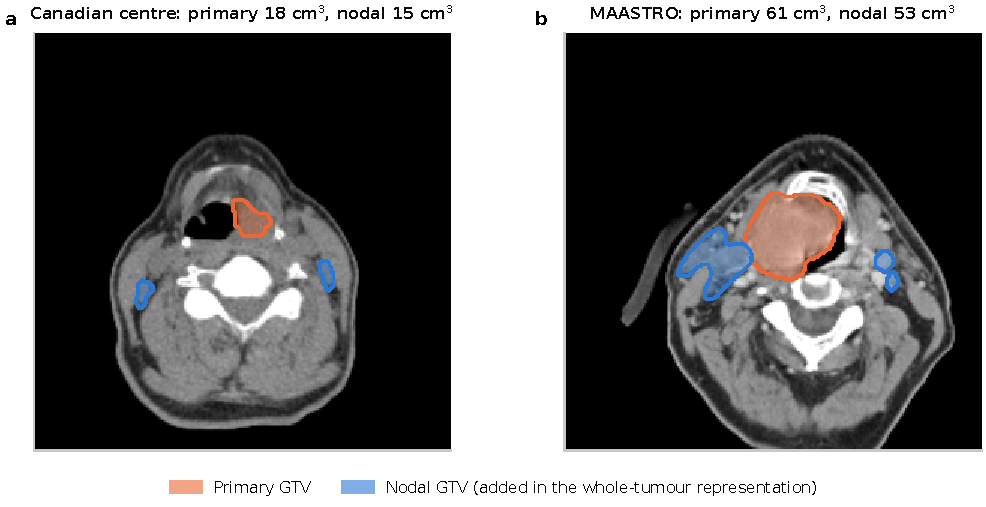
\includegraphics[width=\textwidth]{fig_ct_tumour.pdf}
\caption{Tumour definitions on pretreatment CT. Axial slices of one Canadian (\textbf{a}) and one MAASTRO (\textbf{b}) patient with the primary GTV (orange), which defined the radiomic region of the earlier analysis, and the nodal GTVs (blue), which are added in the whole-tumour representation. Volumes refer to the whole structures.}\label{fig:ct}
\end{figure}

\subsection{Clinical variables}
The clinical variables were those of the CNN with clinical data~\cite{mateus2023}: T category (T1--T4), N category (N0, N1, N2 or higher) and the GTV volume in four bins with their cut-offs (11, 24 and 43\,cm$^3$). Two variants were compared. In the first, the volume bins were computed from the GTV used for the radiomic features; in the second (tumour burden), they were computed from the total GTV and complemented by the logarithm of the nodal GTV volume and the number of nodal GTV structures, capped at four.

\subsection{Population graph and models}
For every split, the patients of the training, validation and test sets formed the nodes of one population graph (Fig.~\ref{fig:graph}). Node features were the radiomic features chosen by a selector fitted on the training patients, optionally concatenated with the clinical variables. Features were median-imputed, log-transformed when heavy-tailed (absolute skewness above 2), z-scored and clipped at $\pm5$ standard deviations with statistics of the training patients. Edges were built inductively: every node received directed edges from its $k$ most similar training patients by cosine similarity of the node features, and training nodes were not linked to themselves through this rule. Validation and test patients therefore had no outgoing edges, so that their predictions depended only on their own features and those of training patients, and no label of a validation or test patient could reach any other node.

Three graph neural networks were compared: a graph convolutional network (GCN)~\cite{kipf2017gcn}, GraphSAGE~\cite{hamilton2017graphsage} and a graph attention network (GAT, four heads)~\cite{velickovic2018gat}. Each had two message-passing layers with 32 hidden units, exponential linear units, a linear skip connection from the input, a residual connection between the layers, input dropout of 0.2 and hidden dropout of 0.5, and a linear output. The control was the identical network in which both message-passing layers were replaced by linear layers, that is, a multilayer perceptron (MLP) that sees exactly the same node features but no edges. Networks were trained full-batch for 150 epochs with Adam (learning rate $5\times10^{-3}$, weight decay $5\times10^{-3}$) and a binary cross-entropy loss weighted by the inverse class ratio of the training patients. Every configuration was trained with ten seeds (0--9) and the predicted probabilities were averaged.

\begin{figure}[!htb]
\centering
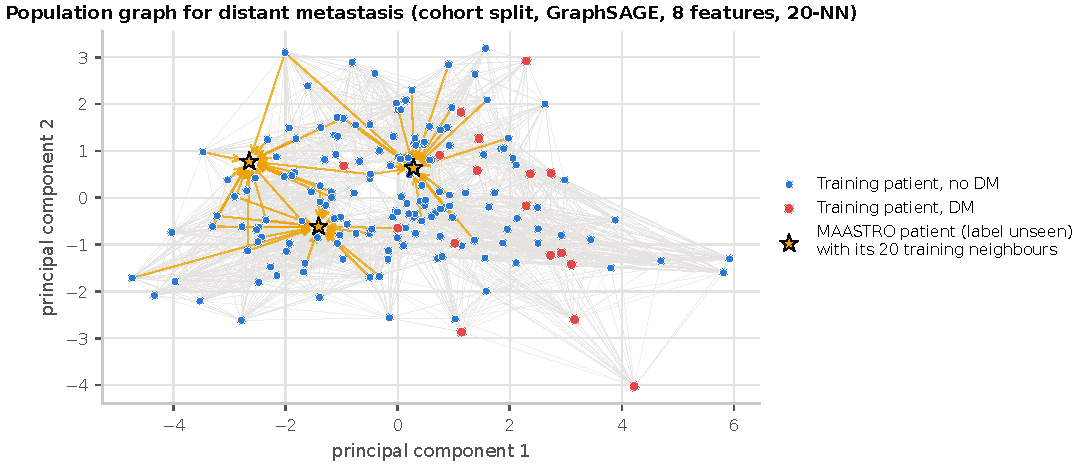
\includegraphics[width=\textwidth]{fig_population_graph.pdf}
\caption{Population graph of the distant-metastasis model chosen in the cohort split with imaging inputs, shown in the first two principal components of its node features. Every training patient (blue: no DM; red: DM) receives edges from its \figGraphK{} most similar training patients (grey). Three MAASTRO patients (stars) are shown with their incoming edges (orange); test patients receive edges only from training patients and send none, so that no test label or test feature reaches another node.}\label{fig:graph}
\end{figure}

\subsection{Configuration grid and model selection}
For each endpoint, design and input set, the grid crossed two feature sets (the 107 original and shape features, or all 479 features), three selectors fitted on the training patients (minimum-redundancy maximum-relevance~\cite{peng2005mrmr}, LASSO~\cite{tibshirani1996lasso}, and a univariate filter that ranks features by their training AUC and discards any feature correlated at $|r|\geq0.8$ with a better-ranked one), three subset sizes ($k=2$, 4 and 8), three neighbourhood sizes (5, 10 and 20 training neighbours) and the four networks, which gave 162 graph configurations and 18 MLP configurations per input set. Imaging-only and imaging-with-clinical inputs were analysed separately, as in the CNN study, and a clinical-only graph was trained as a reference. The configuration with the highest validation AUC (pooled out-of-fold predictions in CV, the validation centres in the cohort split) was chosen separately for the graph networks and for the MLP. To determine whether the graph helps, the two choices were compared on MAASTRO, and every graph configuration was also compared with the MLP that used identical features (same feature set, selector, subset size and input set).

\subsection{Conventional classifiers}
To place the networks in context, conventional classifiers were trained on the same whole-tumour features and splits with the grid of the earlier GTV-only analysis: three feature sets (original, original and shape, all), the same three selectors, five subset sizes ($k=2$, 4, 6, 10 and 15) and five classifiers (L2-penalised logistic regression with $C=0.03$, 0.3 or 3, and random forests of 500 trees with maximum depth 3 or 6, both with balanced class weights~\cite{pedregosa2011sklearn,breiman2001rf}), with and without the clinical variables of the earlier analysis (age, sex, HPV status, T and N category, subsite and concurrent chemotherapy). Logistic regression ($C=0.3$) on the GTV volume alone, on the clinical variables alone and on both together was included as a reference. The configuration with the highest validation AUC was chosen in the same way, among all models with the respective inputs.

\subsection{Representation ablation}
The contribution of the tumour definition and of tumour burden was separated with a $2\times2$ ablation in which the complete grid was rerun for each combination of radiomic features (primary GTV or whole tumour) and clinical variables (volume bins only, or tumour burden). The whole-tumour representation was motivated by the composition of the CNN input and introduced after the primary-GTV results were known; the four representations are therefore reported in full rather than only the best.

\subsection{Statistical analysis}
Discrimination was measured by the area under the receiver operating characteristic curve (AUC). External results are reported in the format of Mateus et al.~\cite{mateus2023}: in CV, the mean and range of the five per-fold MAASTRO AUCs, and in the cohort split, the MAASTRO AUC with a 95\% percentile bootstrap confidence interval (1000 resamples)~\cite{efron1993}. The CNN values were taken from Tables 3 (imaging) and 4 (with clinical data) of their report; because their predictions are not available, the comparison with the CNN is descriptive. The chosen graph network and the chosen MLP were compared on MAASTRO with a paired patient-level bootstrap of the AUC difference (2000 resamples; CV predictions averaged over the five fold models). To quantify the influence of training randomness, every chosen configuration was retrained with ten further, disjoint blocks of ten seeds (seeds from 1000 onwards), each block a complete re-run of the ensemble, and the spread of the external AUC across the re-runs was recorded. Analyses used PyTorch~\cite{paszke2019pytorch}, PyTorch Geometric~\cite{fey2019pyg} and scikit-learn~\cite{pedregosa2011sklearn}.

%% =========================================================================================
\section{Results}\label{sec:results}

\subsection{Cohorts and tumour burden}
The development cohort comprised \nPatCan{} and the test cohort \nPatMAA{} patients with delineations; after the endpoint-specific exclusions, MAASTRO contributed \nTestLR{} patients with \eTestLR{} LR events, \nTestDM{} with \eTestDM{} DM events and \nTestOS{} with \eTestOS{} deaths. The two cohorts differed markedly in how the tumour had been delineated (Table~\ref{tab:burden}, Fig.~\ref{fig:ct}). Separate nodal GTVs were present in \nodalPctCan\% of Canadian but \nodalPctMAA\% of MAASTRO patients, although node-positive disease was common in both, and the Canadian primary GTVs were larger (median 23.8 versus 14.1\,cm$^3$). The difference was concentrated in one centre: HGJ had separate nodal GTVs in only 12\% of its patients although 89\% were node positive, and its primary GTVs were the largest of the four centres, and several Canadian structures labelled as the primary tumour were named as tumour and nodes together. The primary GTV therefore did not describe the same anatomy in the development and test cohorts, whereas the union of the primary and nodal GTVs described the whole delineated tumour in both.

\begin{table}[!htb]
\centering
\caption{Tumour burden by cohort. Volumes are median (interquartile range) over patients with delineations; nodal GTVs are the structures listed as nodal in the Head-Neck-PET-CT index and GTV-2 to GTV-$n$ in HN1.}\label{tab:burden}
\small
\begin{tabular}{@{}lll@{}}
\toprule
Tumour burden & Canadian centres & MAASTRO (HN1) \\
\midrule
Patients with delineations & 294 & 137 \\
Patients with nodal GTV, n (\%) & 110 (37\%) & 81 (59\%) \\
Primary GTV, cm$^3$ & 23.8 (12.0--40.8) & 14.1 (3.7--33.7) \\
Nodal GTV (if present), cm$^3$ & 15.7 (6.1--34.7) & 10.5 (4.9--26.4) \\
Total GTV, cm$^3$ & 31.3 (16.4--54.0) & 20.1 (6.6--52.1) \\
Nodal share of total GTV, median & 0\% & 14\% \\
Nodal share when nodes present, median & 44\% & 30\% \\
\botrule
\end{tabular}

\end{table}

\subsection{External discrimination of the whole-tumour models}
With whole-tumour radiomic features and tumour-burden clinical variables, the population graph networks chosen on validation reached external AUCs of \mainLRMin--\mainLRMax{} for LR, \mainDMMin--\mainDMMax{} for DM and \mainOSMin--\mainOSMax{} for OS (Table~\ref{tab:main}, Fig.~\ref{fig:auc}), and exceeded the CNN of Mateus et al.\ in \winsGraph{} of the 12 settings. For LR, the graph networks exceeded the CNN in all four settings, most clearly in the cohort split with imaging only (\mainLRCohImg{} [\mainCILRCohImg] versus \cnnLRCohImg), where the CNN had performed below chance. For OS they also exceeded the CNN in all four settings, by 0.01 to 0.10, the largest difference occurring in CV with imaging only (\mainOSCVImg{} versus \cnnOSCVImg). For DM, the graph network exceeded the CNN in CV with imaging only (\mainDMCVImg{} versus \cnnDMCVImg) and was within 0.02 of it in CV with clinical data and in the cohort split with imaging only, but it remained below the CNN in the cohort split with clinical data (\mainDMCohClin{} [\mainCIDMCohClin] versus \cnnDMCohClin); the confidence interval included the CNN value, and the DM test set contained only \eTestDM{} events. A graph network on the clinical variables alone reached \clinOnlyLRMin--\clinOnlyLRMax{} for LR, \clinOnlyDMMin--\clinOnlyDMMax{} for DM and \clinOnlyOSMin--\clinOnlyOSMax{} for OS, so that the radiomic features added most for LR and DM and little for OS. The chosen configurations are listed in Supplementary Table~\ref{tab:configs}.

\begin{table}[!htb]
\centering
\caption{External discrimination on MAASTRO (HN1) of the whole-tumour models chosen on validation, compared with the CNN. CV: mean (range) of the five per-fold AUCs; cohort split: AUC [95\% bootstrap confidence interval]. Bold: above the CNN.}\label{tab:main}
\scriptsize
\setlength{\tabcolsep}{3pt}
\begin{tabular}{@{}lllllll@{}}
\toprule
Endpoint & Design & Inputs & CNN$^{a}$ & Population GNN$^{b}$ & MLP, no graph$^{b}$ & Logistic/RF$^{c}$ \\
\midrule
Locoregional recurrence & 5-fold CV & Imaging & 0.53 & GAT \textbf{0.62} (0.52--0.68) & \textbf{0.59} (0.55--0.62) & -- \\
 &  & Imaging + clinical & 0.57 & GraphSAGE \textbf{0.59} (0.53--0.65) & \textbf{0.59} (0.50--0.64) & -- \\
 & Cohort split & Imaging & 0.45 & GCN \textbf{0.63} [0.51, 0.74] & \textbf{0.64} [0.52, 0.75] & -- \\
 &  & Imaging + clinical & 0.59 & GCN \textbf{0.60} [0.46, 0.72] & 0.58 [0.45, 0.71] & -- \\
\midrule
Distant metastasis & 5-fold CV & Imaging & 0.83 & GCN \textbf{0.85} (0.82--0.86) & \textbf{0.85} (0.81--0.87) & -- \\
 &  & Imaging + clinical & 0.88 & GraphSAGE 0.87 (0.85--0.88) & 0.86 (0.85--0.88) & -- \\
 & Cohort split & Imaging & 0.89 & GraphSAGE 0.87 [0.71, 0.99] & 0.86 [0.70, 0.99] & -- \\
 &  & Imaging + clinical & 0.93 & GCN 0.85 [0.68, 0.98] & 0.86 [0.71, 0.97] & -- \\
\midrule
Overall survival & 5-fold CV & Imaging & 0.63 & GCN \textbf{0.73} (0.72--0.75) & \textbf{0.74} (0.74--0.75) & -- \\
 &  & Imaging + clinical & 0.68 & GCN \textbf{0.72} (0.70--0.74) & \textbf{0.72} (0.71--0.73) & -- \\
 & Cohort split & Imaging & 0.67 & GraphSAGE \textbf{0.72} [0.61, 0.82] & \textbf{0.73} [0.63, 0.83] & -- \\
 &  & Imaging + clinical & 0.69 & GraphSAGE \textbf{0.70} [0.58, 0.80] & \textbf{0.72} [0.61, 0.81] & -- \\
\botrule
\end{tabular}

\tabnote{$^{a}$Mateus et al.~\cite{mateus2023}, Tables 3 and 4. $^{b}$Whole-tumour features and tumour-burden clinical variables; the population GNN is the best of GCN, GraphSAGE and GAT on validation, and the MLP is the same network without edges, chosen separately. $^{c}$L2-penalised logistic regression or random forest on the same whole-tumour features with the clinical variables of the earlier analysis, chosen on validation.}
\end{table}

\begin{figure}[!htb]
\centering
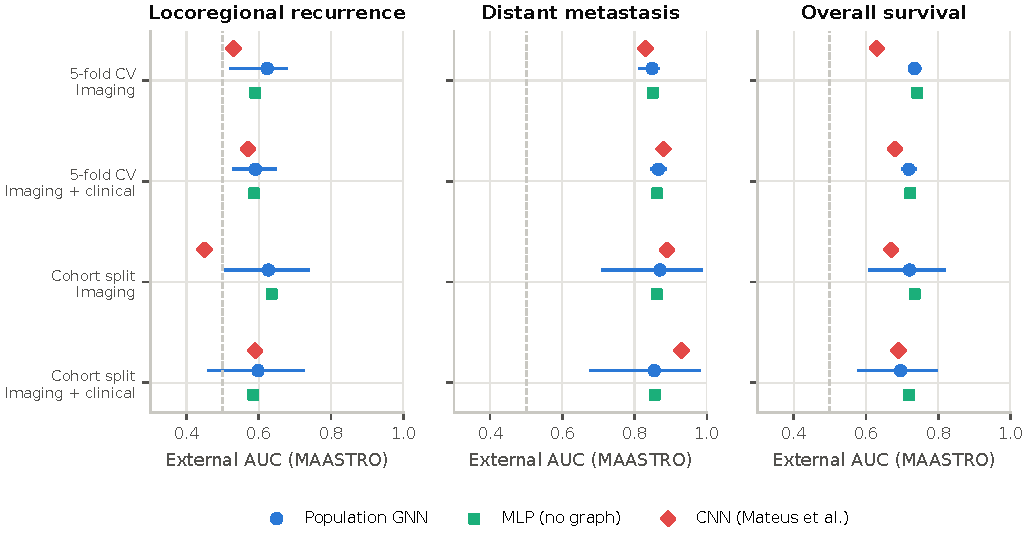
\includegraphics[width=\textwidth]{fig_auc_vs_cnn.pdf}
\caption{External AUC on MAASTRO of the population graph network (circles; CV: range of per-fold AUCs, cohort split: 95\% bootstrap confidence interval) and of the MLP without edges (squares), both on whole-tumour features and chosen on validation, compared with the published CNN (diamonds)~\cite{mateus2023}. The dashed line marks chance.}\label{fig:auc}
\end{figure}

\subsection{Tumour definition versus tumour burden}
The $2\times2$ ablation separated the two changes (Table~\ref{tab:ablation}, Fig.~\ref{fig:ablation}). With primary-GTV features, the graph networks exceeded the CNN in \winsPrimVol{} of 12 settings with the volume bins and in \winsPrimBur{} of 12 with the tumour-burden variables, and they were 0.04 to 0.28 below the CNN for DM in every setting. With whole-tumour features, they exceeded the CNN in \winsTotVol{} of 12 settings with the volume bins and in \winsTotBur{} of 12 with the tumour-burden variables. The tumour definition was therefore responsible for the improvement: it raised the DM AUC from \ablPrimVolDMMin--\ablPrimVolDMMax{} to \ablTotVolDMMin--\ablTotVolDMMax{} and the OS AUC from \ablPrimVolOSMin--\ablPrimVolOSMax{} to \ablTotVolOSMin--\ablTotVolOSMax, and left LR unchanged (\ablPrimVolLRMin--\ablPrimVolLRMax{} and \ablTotVolLRMin--\ablTotVolLRMax). Tumour-burden variables improved the DM AUC of the primary-GTV models when combined with imaging (from \ablPrimVolDMMax{} to \ablPrimBurDMMax{} at most), which confirms that nodal burden carries prognostic information for distant failure, but added nothing once the nodal tumour was part of the radiomic region.

\begin{table}[!htb]
\centering
\caption{Representation ablation: external AUC on MAASTRO of the population graph network chosen on validation for each combination of radiomic region and clinical variables. CV: mean of the per-fold AUCs; cohort: pooled AUC. Bold: above the CNN. Img: imaging; +Cl: imaging and clinical.}\label{tab:ablation}
\scriptsize
\setlength{\tabcolsep}{2.6pt}
\begin{tabular}{@{}llccccccccccccc@{}}
\toprule
 & & \multicolumn{4}{c}{LR} & \multicolumn{4}{c}{DM} & \multicolumn{4}{c}{OS} & \\
\cmidrule(lr){3-6}\cmidrule(lr){7-10}\cmidrule(lr){11-14}
 & & \multicolumn{2}{c}{CV} & \multicolumn{2}{c}{Cohort} & \multicolumn{2}{c}{CV} & \multicolumn{2}{c}{Cohort} & \multicolumn{2}{c}{CV} & \multicolumn{2}{c}{Cohort} & \\
Tumour region & Clinical & Img & +Cl & Img & +Cl & Img & +Cl & Img & +Cl & Img & +Cl & Img & +Cl & Wins \\
\midrule
CNN (Mateus et al.) & -- & 0.53 & 0.57 & 0.45 & 0.59 & 0.83 & 0.88 & 0.89 & 0.93 & 0.63 & 0.68 & 0.67 & 0.69 & -- \\
\midrule
Primary GTV & T, N, volume & \textbf{0.61} & \textbf{0.58} & \textbf{0.63} & \textbf{0.63} & 0.65 & 0.78 & 0.70 & 0.65 & \textbf{0.67} & \textbf{0.70} & 0.65 & 0.67 & 6/12 \\
Primary GTV & T, N, burden & \textbf{0.61} & \textbf{0.58} & \textbf{0.63} & \textbf{0.60} & 0.65 & 0.84 & 0.70 & 0.72 & \textbf{0.67} & \textbf{0.69} & 0.65 & \textbf{0.69} & 7/12 \\
Primary + nodal GTV & T, N, volume & \textbf{0.62} & \textbf{0.58} & \textbf{0.63} & \textbf{0.61} & \textbf{0.85} & 0.88 & 0.87 & 0.86 & \textbf{0.73} & \textbf{0.72} & \textbf{0.72} & \textbf{0.72} & 9/12 \\
Primary + nodal GTV & T, N, burden & \textbf{0.62} & \textbf{0.59} & \textbf{0.63} & \textbf{0.60} & \textbf{0.85} & 0.87 & 0.87 & 0.85 & \textbf{0.73} & \textbf{0.72} & \textbf{0.72} & \textbf{0.70} & 9/12 \\
\botrule
\end{tabular}

\end{table}

\begin{figure}[!htb]
\centering
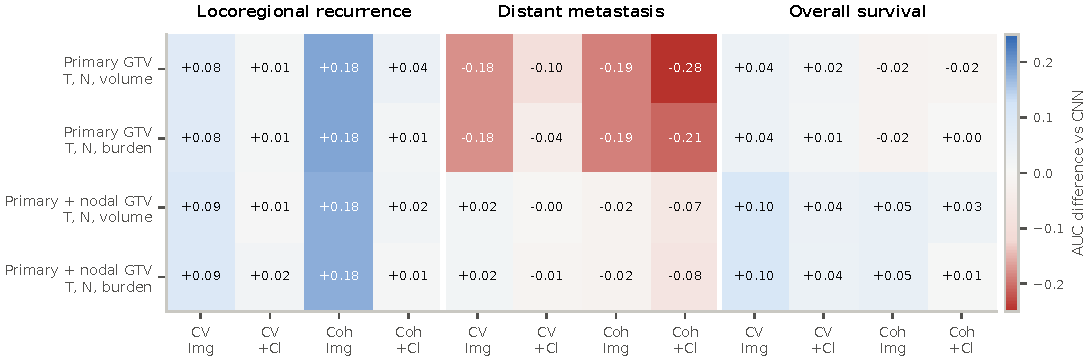
\includegraphics[width=\textwidth]{fig_ablation.pdf}
\caption{Difference between the external AUC of the chosen population graph network and that of the CNN~\cite{mateus2023} for every combination of radiomic region (rows: primary GTV or primary and nodal GTV) and clinical variables (volume bins or tumour burden), endpoint, design (CV, Coh: cohort split) and inputs (Img: imaging; +Cl: imaging and clinical). Blue: above the CNN; red: below.}\label{fig:ablation}
\end{figure}

\subsection{Does the patient graph help?}
The MLP, which used the same node features and layers but no edges, exceeded the CNN in \winsMLP{} of the 12 settings, against \winsGraph{} for the graph networks (Table~\ref{tab:main}). The external AUCs of the graph network and of the MLP chosen on validation differed by \pairedDeltaMin{} to \pairedDeltaMax{} across the \pairedN{} endpoint, design and input combinations, including the clinical-only models (Table~\ref{tab:paired}). Only one difference reached nominal significance ($p=\pairedMinP$), and it favoured the MLP. The matched comparison gave the same answer (Fig.~\ref{fig:matched}). Of the \matchedN{} graph configurations, each compared with the MLP that used exactly the same features, the graph network had the higher validation AUC in \matchedValFracAll\% and the higher external AUC in \matchedTestFracAll\%, with a median external difference of \matchedTestMedAll. The graph was least harmful for LR, where the graph network was better on MAASTRO in \matchedTestFracLR\% of matched comparisons, and most harmful for OS (\matchedTestFracOS\%). The improvement over the CNN therefore lay in the node features, and the edges between patients did not add to it.

\begin{table}[!htb]
\centering
\caption{Paired comparison on MAASTRO of the graph network and the MLP without edges, each chosen on validation with whole-tumour features. $\Delta$AUC: graph minus MLP with 95\% paired bootstrap confidence interval (2000 resamples; CV predictions averaged over the five fold models) and two-sided bootstrap $p$ value.}\label{tab:paired}
\scriptsize
\setlength{\tabcolsep}{3.5pt}
\begin{tabular}{@{}lllllll@{}}
\toprule
Design & Inputs & Graph model & Graph AUC & MLP AUC & $\Delta$AUC [95\% CI] & $p$ \\
\midrule
\multicolumn{7}{@{}l}{\textit{Locoregional recurrence}} \\
5-fold CV & Imaging & GAT & 0.666 & 0.616 & +0.050 [$-$0.050, +0.150] & 0.38 \\
 & Imaging + clinical & GraphSAGE & 0.615 & 0.605 & +0.010 [$-$0.041, +0.066] & 0.72 \\
 & Clinical & GCN & 0.576 & 0.570 & +0.006 [$-$0.019, +0.032] & 0.65 \\
Cohort split & Imaging & GCN & 0.627 & 0.636 & $-$0.009 [$-$0.045, +0.027] & 0.63 \\
 & Imaging + clinical & GCN & 0.598 & 0.585 & +0.013 [$-$0.024, +0.053] & 0.52 \\
 & Clinical & GAT & 0.507 & 0.478 & +0.029 [$-$0.011, +0.069] & 0.17 \\
\midrule
\multicolumn{7}{@{}l}{\textit{Distant metastasis}} \\
5-fold CV & Imaging & GCN & 0.882 & 0.878 & +0.004 [$-$0.009, +0.022] & 0.72 \\
 & Imaging + clinical & GraphSAGE & 0.867 & 0.873 & $-$0.006 [$-$0.028, +0.013] & 0.66 \\
 & Clinical & GAT & 0.829 & 0.843 & $-$0.014 [$-$0.051, +0.013] & 0.38 \\
Cohort split & Imaging & GraphSAGE & 0.870 & 0.861 & +0.008 [$-$0.014, +0.033] & 0.51 \\
 & Imaging + clinical & GCN & 0.854 & 0.856 & $-$0.001 [$-$0.031, +0.031] & 0.91 \\
 & Clinical & GCN & 0.793 & 0.814 & $-$0.021 [$-$0.063, +0.012] & 0.28 \\
\midrule
\multicolumn{7}{@{}l}{\textit{Overall survival}} \\
5-fold CV & Imaging & GCN & 0.741 & 0.744 & $-$0.004 [$-$0.018, +0.011] & 0.64 \\
 & Imaging + clinical & GCN & 0.720 & 0.723 & $-$0.003 [$-$0.017, +0.012] & 0.72 \\
 & Clinical & GAT & 0.692 & 0.715 & $-$0.023 [$-$0.047, $-$0.001] & 0.03 \\
Cohort split & Imaging & GraphSAGE & 0.721 & 0.735 & $-$0.014 [$-$0.051, +0.021] & 0.38 \\
 & Imaging + clinical & GraphSAGE & 0.696 & 0.719 & $-$0.023 [$-$0.055, +0.005] & 0.13 \\
 & Clinical & GCN & 0.701 & 0.704 & $-$0.003 [$-$0.029, +0.023] & 0.79 \\
\botrule
\end{tabular}

\end{table}

\begin{figure}[!htb]
\centering
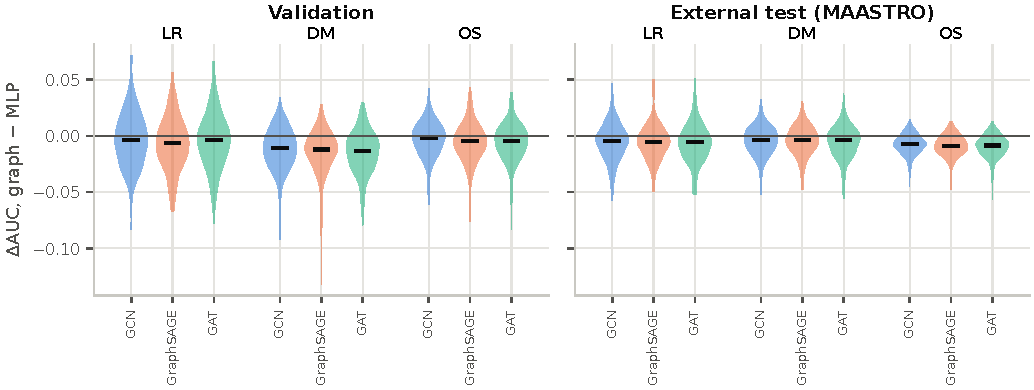
\includegraphics[width=\textwidth]{fig_graph_vs_mlp.pdf}
\caption{Matched comparison of every graph configuration with the MLP that used identical features (feature set, selector, subset size and inputs), on validation (left) and on MAASTRO (right), by endpoint and graph network. Values above zero favour the graph. Horizontal lines within the violins mark medians.}\label{fig:matched}
\end{figure}

\subsection{Training randomness and conventional classifiers}
When every chosen configuration was retrained with \seedRepeats{} disjoint ten-seed ensembles, the standard deviation of the external AUC across the re-runs had a median of \seedSDmed{} and a maximum of \seedSDmax{} (Fig.~\ref{fig:seed}, Supplementary Table~\ref{tab:seed}). The graph network exceeded the CNN in every re-run in \seedStableWins{} of the 12 settings and in none in \seedStableLoss, so that the comparison with the CNN did not depend on the seeds used for the reported models. Conventional classifiers on the same whole-tumour features, with the clinical variables of the earlier analysis, reached external AUCs of \clsLRMin--\clsLRMax{} for LR, \clsDMMin--\clsDMMax{} for DM and \clsOSMin--\clsOSMax{} for OS and also exceeded the CNN in \winsCls{} of the 12 settings (Table~\ref{tab:main}). With imaging alone they were similar to the graph networks for DM and OS and lower for LR, but with clinical data they reached \clsLRCVClin{} and \clsLRCohClin{} for LR, well above the graph networks. This difference came from the clinical variables rather than from the radiomic features: logistic regression on these clinical variables alone, which include age, human papillomavirus (HPV) status and tumour subsite in addition to T and N category, reached \clsClinLRMin--\clsClinLRMax{} for LR, \clsClinDMMin--\clsClinDMMax{} for DM and \clsClinOSMin--\clsClinOSMax{} for OS, and in the cohort split for LR the configuration chosen with clinical inputs was the clinical model with GTV volume and no texture features. The graph networks, in contrast, used the clinical variables of the CNN study, which contain neither age nor HPV status.

\begin{figure}[!htb]
\centering
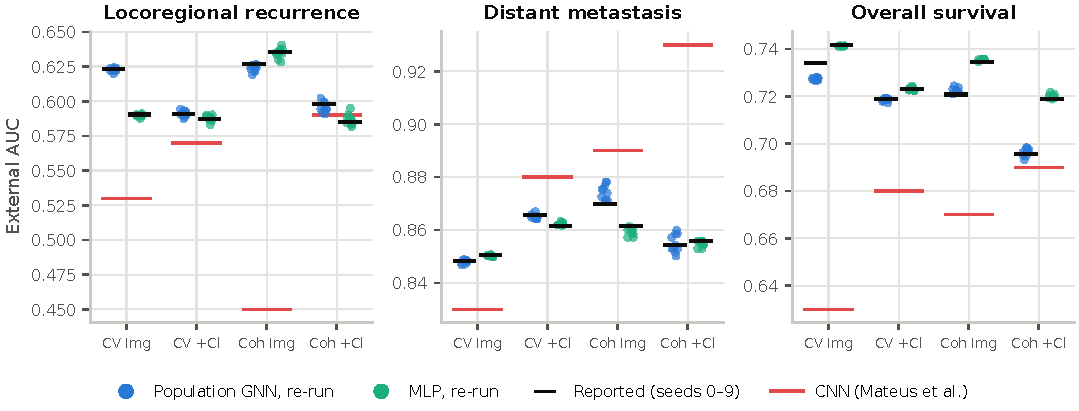
\includegraphics[width=\textwidth]{fig_seed.pdf}
\caption{External AUC on MAASTRO of the chosen graph networks (blue) and MLPs (green) when retrained with disjoint ten-seed ensembles, by endpoint, design (CV, Coh: cohort split) and inputs (Img: imaging; +Cl: imaging and clinical). Black bars: reported models (seeds 0--9); red lines: CNN~\cite{mateus2023}.}\label{fig:seed}
\end{figure}

%% =========================================================================================
\section{Discussion}\label{sec:discussion}

Under the public protocol of Mateus et al., population graph networks on radiomic features of the whole tumour matched or exceeded the published CNN for LR and OS and came close to it for DM, whereas the same networks on the primary GTV fell well short for DM. The ablation attributed this difference to the tumour definition and not to tumour burden as a clinical variable, and the comparison with the identical network without edges showed that the patient graph contributed nothing: the MLP reached the same external discrimination, the paired differences were small and not systematically in favour of the graph, and with identical features the graph network was more often worse than better.

The importance of the tumour definition has two explanations, and the data support both. The first is biological. Nodal disease and the total tumour volume are among the strongest predictors of distant metastasis in HNSCC~\cite{kjems2023volume,jensen2020nodalfdg}, and a radiomic description of the primary tumour alone cannot capture them; the CNN, which received the whole image, could. The second is a measurement artefact. Separate nodal GTVs were delineated in \nodalPctCan\% of the Canadian but \nodalPctMAA\% of the MAASTRO patients, and in one Canadian centre nodal disease appears to have been included in the structure designated as the primary GTV. A model trained on the primary GTV therefore learnt from a structure that partly contained nodes and was tested on one that did not, so that a part of its DM signal could not transfer. Taking the union of all GTVs removes this inconsistency, because the whole delineated tumour is described in the same way whatever its subdivision. The two explanations cannot be fully separated with these data, but both lead to the same recommendation: radiomic models compared with image-based deep learning should be built on the same tumour region as the network sees, and the consistency of delineation conventions across public cohorts should be checked before features are compared.

The negative result for the graph agrees with what is known about population graphs. Their reported gains in neuroimaging and in COVID-19 pneumonia were obtained with richer non-imaging data used to define the edges and were seldom compared with an equally tuned network without edges~\cite{parisot2018population,keicher2023covid}. Here the edges were defined by the same features as the nodes, so that message passing could only smooth each patient's prediction towards those of similar training patients, which an MLP with the same features can approximate. With a few hundred patients and a handful of selected features, such smoothing offers no information that the features do not already contain. This conclusion would have been missed without the no-edge control: the graph networks did exceed the CNN in \winsGraph{} of 12 settings, and in isolation this could have been attributed to the graph. Population graph studies should therefore report the identical network without edges as a matter of course.

The conventional classifiers placed these results in perspective. On the same whole-tumour features, logistic regression and random forests did as well as the graph networks, which again indicates that the gain lay in the features, and for LR a richer clinical description, including age and HPV status, outperformed every imaging model and the CNN. The comparison with the CNN in this study was deliberately restricted to the clinical variables that the CNN had used, so that the radiomic and deep learning models received the same information; it should not be read as evidence that imaging adds to a complete clinical model for LR, which these data do not support.

The results also extend the earlier GRAFS-GAT analysis on the same protocol~\cite{shaikh2026grafs}, in which neither feature selection nor graph topology changed external discrimination materially and the random seed was the largest source of variance. In the present study the networks were trained as ten-seed ensembles, and the re-runs with disjoint seed blocks varied by a few thousandths of an AUC at most, so that ensembling removed the seed dependence that had dominated single networks and the comparison with the CNN did not change between re-runs. Together, the two analyses suggest that, for CT radiomics in HNSCC cohorts of this size, the choice of what is measured matters more than the architecture that combines the measurements.

The study has limitations. First, the whole-tumour representation was introduced after the primary-GTV results had been seen, so that the MAASTRO data were used more than once; this risk was reduced by the \emph{a priori} motivation from the composition of the CNN input, by choosing every model on validation data only, and by reporting all four representations of the ablation rather than the best, but the whole-tumour results should be confirmed in an independent cohort. Second, the DM test set contained only \eTestDM{} events, so that the DM AUCs have wide confidence intervals and differences of several hundredths cannot be resolved. Third, the comparison with the CNN is descriptive, because its predictions are not available for a paired test. Fourth, nodal delineations in public collections are incomplete and their conventions undocumented, so that the whole tumour as defined here depends on what each centre chose to contour. Finally, only CT radiomics was studied, and edges based on other data, such as genomics or PET, might behave differently.

%% =========================================================================================
\section{Conclusion}\label{sec:conclusion}
Population graph neural networks on radiomic features of the whole tumour, the primary and nodal GTVs together, matched or exceeded a published CNN for locoregional recurrence and overall survival and approached it for distant metastasis under the same public protocol, whereas the same networks on the primary GTV did not. The improvement came from the tumour definition, which captures nodal disease and harmonises inconsistent delineations across cohorts, and not from the patient graph, which added nothing over the identical network without edges. For locoregional recurrence, clinical variables including HPV status outperformed all imaging models. Radiomic models should describe the same tumour region as the image-based models they are compared with, imaging models should be compared with a complete clinical model, and population graph studies should report the no-edge control.

%% =========================================================================================
\section*{Declarations}

\paragraph{Supplementary information.}The appendix lists the configurations chosen on validation and the results of the seed re-runs.

\paragraph{Acknowledgements.}The author thanks the investigators who made the Head-Neck-PET-CT and HN1 collections publicly available through The Cancer Imaging Archive.

\paragraph{Funding.}[To be completed; state ``No funding was received for this study'' if applicable.]

\paragraph{Competing interests.}The author declares no competing interests.

\paragraph{Ethics approval and consent to participate.}This study analysed de-identified, publicly available data from The Cancer Imaging Archive. The original studies obtained institutional ethics approval and informed consent or a waiver, and no additional approval was required for this secondary analysis. [Confirm with the institutional ethics committee.]

\paragraph{Consent for publication.}Not applicable.

\paragraph{Data availability.}The Head-Neck-PET-CT (\url{https://doi.org/10.7937/K9/TCIA.2017.8oje5q00}) and HN1 (\url{https://doi.org/10.7937/tcia.2019.8kap372n}) collections are available from The Cancer Imaging Archive.

\paragraph{Code availability.}The feature extraction, population graph, ablation and analysis code and the script that generates every table and figure are available at \url{https://github.com/hash123shaikh/Radiomics_Graph_Attention_Network_HNC} (directory \texttt{grafs-gat/popgraph}).

\paragraph{Author contribution.}The author conceived and designed the study, implemented the software, performed all analyses, interpreted the results and wrote the manuscript.

\bibliographystyle{unsrtnat}
{\small
\bibliography{references}}

%% =========================================================================================
\clearpage
\appendix
\renewcommand{\thetable}{S\arabic{table}}
\setcounter{table}{0}
\section*{Appendix}

\begin{table}[!htb]
\centering
\caption{Configurations chosen on validation for every endpoint, design and input set, separately for the graph networks and for the MLP without edges. Features: original + shape (107) or all including Laplacian-of-Gaussian features (479); $k$: number of selected radiomic features; graph: number of training neighbours per node.}\label{tab:configs}
\scriptsize
\setlength{\tabcolsep}{3pt}
\begin{tabular}{@{}lllllllll@{}}
\toprule
Endpoint & Design & Inputs & Family & Features & Selector & $k$ & Graph & Val.\ AUC \\
\midrule
LR & 5-fold CV & Imaging & GAT & original + shape & LASSO & 2 & 20-NN & 0.567 \\
LR & 5-fold CV & Imaging & MLP & all (incl.\ LoG) & mRMR & 2 & -- & 0.577 \\
LR & 5-fold CV & Imaging + clinical & GraphSAGE & original + shape & LASSO & 4 & 5-NN & 0.638 \\
LR & 5-fold CV & Imaging + clinical & MLP & original + shape & LASSO & 4 & -- & 0.581 \\
LR & 5-fold CV & Clinical & GCN & -- & -- & -- & 20-NN & 0.560 \\
LR & 5-fold CV & Clinical & MLP & -- & -- & -- & -- & 0.535 \\
LR & Cohort split & Imaging & GCN & original + shape & LASSO & 2 & 20-NN & 0.559 \\
LR & Cohort split & Imaging & MLP & original + shape & LASSO & 2 & -- & 0.537 \\
LR & Cohort split & Imaging + clinical & GCN & original + shape & LASSO & 4 & 10-NN & 0.592 \\
LR & Cohort split & Imaging + clinical & MLP & original + shape & LASSO & 4 & -- & 0.559 \\
LR & Cohort split & Clinical & GAT & -- & -- & -- & 10-NN & 0.648 \\
LR & Cohort split & Clinical & MLP & -- & -- & -- & -- & 0.633 \\
\midrule
DM & 5-fold CV & Imaging & GCN & original + shape & univariate & 4 & 5-NN & 0.768 \\
DM & 5-fold CV & Imaging & MLP & original + shape & univariate & 4 & -- & 0.777 \\
DM & 5-fold CV & Imaging + clinical & GraphSAGE & original + shape & univariate & 4 & 20-NN & 0.793 \\
DM & 5-fold CV & Imaging + clinical & MLP & original + shape & univariate & 4 & -- & 0.797 \\
DM & 5-fold CV & Clinical & GAT & -- & -- & -- & 10-NN & 0.732 \\
DM & 5-fold CV & Clinical & MLP & -- & -- & -- & -- & 0.732 \\
DM & Cohort split & Imaging & GraphSAGE & all (incl.\ LoG) & LASSO & 8 & 20-NN & 0.901 \\
DM & Cohort split & Imaging & MLP & all (incl.\ LoG) & LASSO & 8 & -- & 0.895 \\
DM & Cohort split & Imaging + clinical & GCN & all (incl.\ LoG) & LASSO & 8 & 20-NN & 0.886 \\
DM & Cohort split & Imaging + clinical & MLP & all (incl.\ LoG) & LASSO & 8 & -- & 0.886 \\
DM & Cohort split & Clinical & GCN & -- & -- & -- & 10-NN & 0.714 \\
DM & Cohort split & Clinical & MLP & -- & -- & -- & -- & 0.681 \\
\midrule
OS & 5-fold CV & Imaging & GCN & all (incl.\ LoG) & LASSO & 2 & 20-NN & 0.733 \\
OS & 5-fold CV & Imaging & MLP & original + shape & univariate & 2 & -- & 0.719 \\
OS & 5-fold CV & Imaging + clinical & GCN & original + shape & univariate & 2 & 5-NN & 0.719 \\
OS & 5-fold CV & Imaging + clinical & MLP & original + shape & univariate & 2 & -- & 0.715 \\
OS & 5-fold CV & Clinical & GAT & -- & -- & -- & 10-NN & 0.686 \\
OS & 5-fold CV & Clinical & MLP & -- & -- & -- & -- & 0.682 \\
OS & Cohort split & Imaging & GraphSAGE & original + shape & LASSO & 4 & 5-NN & 0.740 \\
OS & Cohort split & Imaging & MLP & original + shape & univariate & 2 & -- & 0.726 \\
OS & Cohort split & Imaging + clinical & GraphSAGE & original + shape & LASSO & 4 & 5-NN & 0.739 \\
OS & Cohort split & Imaging + clinical & MLP & original + shape & LASSO & 2 & -- & 0.716 \\
OS & Cohort split & Clinical & GCN & -- & -- & -- & 5-NN & 0.670 \\
OS & Cohort split & Clinical & MLP & -- & -- & -- & -- & 0.682 \\
\botrule
\end{tabular}

\end{table}

\begin{table}[!htb]
\centering
\caption{External AUC on MAASTRO of the chosen configurations when retrained with disjoint ten-seed ensembles (seeds from 1000 onwards). Reported: the model of Table~\ref{tab:main} (seeds 0--9).}\label{tab:seed}
\scriptsize
\setlength{\tabcolsep}{3pt}
\begin{tabular}{@{}llllllll@{}}
\toprule
Endpoint & Design & Inputs & Family & Reported & Mean (SD) over re-runs & Range & Re-runs above CNN \\
\midrule
LR & 5-fold CV & Imaging & GNN & 0.623 & 0.622 (nan) & 0.622--0.622 & 1/1 \\
LR & 5-fold CV & Imaging & MLP & 0.590 & 0.588 (nan) & 0.588--0.588 & 1/1 \\
LR & 5-fold CV & Imaging + clinical & GNN & 0.591 & 0.589 (nan) & 0.589--0.589 & 1/1 \\
LR & 5-fold CV & Imaging + clinical & MLP & 0.587 & 0.583 (nan) & 0.583--0.583 & 1/1 \\
LR & Cohort split & Imaging & GNN & 0.627 & 0.622 (nan) & 0.622--0.622 & 1/1 \\
LR & Cohort split & Imaging & MLP & 0.636 & 0.638 (nan) & 0.638--0.638 & 1/1 \\
LR & Cohort split & Imaging + clinical & GNN & 0.598 & 0.599 (nan) & 0.599--0.599 & 1/1 \\
LR & Cohort split & Imaging + clinical & MLP & 0.585 & 0.588 (nan) & 0.588--0.588 & 0/1 \\
\midrule
DM & 5-fold CV & Imaging & GNN & 0.848 & 0.848 (nan) & 0.848--0.848 & 1/1 \\
DM & 5-fold CV & Imaging & MLP & 0.850 & 0.850 (nan) & 0.850--0.850 & 1/1 \\
DM & 5-fold CV & Imaging + clinical & GNN & 0.866 & 0.865 (nan) & 0.865--0.865 & 0/1 \\
DM & 5-fold CV & Imaging + clinical & MLP & 0.862 & 0.862 (nan) & 0.862--0.862 & 0/1 \\
DM & Cohort split & Imaging & GNN & 0.870 & 0.871 (nan) & 0.871--0.871 & 0/1 \\
DM & Cohort split & Imaging & MLP & 0.861 & 0.860 (nan) & 0.860--0.860 & 0/1 \\
DM & Cohort split & Imaging + clinical & GNN & 0.854 & 0.859 (nan) & 0.859--0.859 & 0/1 \\
DM & Cohort split & Imaging + clinical & MLP & 0.856 & 0.856 (nan) & 0.856--0.856 & 0/1 \\
\midrule
OS & 5-fold CV & Imaging & GNN & 0.734 & 0.735 (nan) & 0.735--0.735 & 1/1 \\
OS & 5-fold CV & Imaging & MLP & 0.742 & 0.741 (nan) & 0.741--0.741 & 1/1 \\
OS & 5-fold CV & Imaging + clinical & GNN & 0.719 & 0.719 (nan) & 0.719--0.719 & 1/1 \\
OS & 5-fold CV & Imaging + clinical & MLP & 0.723 & 0.723 (nan) & 0.723--0.723 & 1/1 \\
OS & Cohort split & Imaging & GNN & 0.721 & 0.722 (nan) & 0.722--0.722 & 1/1 \\
OS & Cohort split & Imaging & MLP & 0.735 & 0.736 (nan) & 0.736--0.736 & 1/1 \\
OS & Cohort split & Imaging + clinical & GNN & 0.696 & 0.698 (nan) & 0.698--0.698 & 1/1 \\
OS & Cohort split & Imaging + clinical & MLP & 0.719 & 0.719 (nan) & 0.719--0.719 & 1/1 \\
\botrule
\end{tabular}

\end{table}

\end{document}
